\chapter{Padrões Comportamentais}

\section{Chain of Responsibility}

Chain of Responsability propõe criar uma estrutura para 
tratar solicitações feitas por um objeto cliente. As classes 
que tratam as solicitações são chamadas de \textit{handlers}. 
Uma solicitação é passada adiante por uma cadeia de 
\textit{handlers} até que seja tratada ou 
até que a cadeia chegue ao fim, retornando uma 
indicação de que a solicitação não pôde ser atendida.

Essa abordagem permite desacoplar os clientes das classes 
que tratam as solicitações e permite que os \textit{handlers} 
sejam definidos dinamicamente. Por outro lado, pode não ser 
possível prever se uma solicitação de um cliente será atendida, 
caso um \textit{handler} adequado não esteja na cadeia. A 
estrutura do padrão pode ser vista na figura \ref{chain_struct}.

\begin{figure}[htb]
	\caption{\label{chain_struct}Estrutura do Chain of Responsibility}
	\begin{center}
	    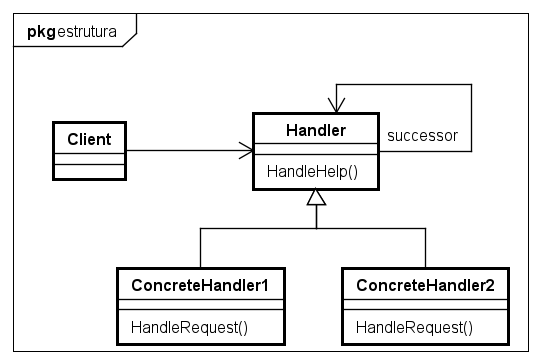
\includegraphics[scale=0.5]{5_padroes-contexto-funcional/5.3_comportamentais/5.3.01_chain-of-responsibility/chainofresponsibility_struct.png}
	\end{center}
\end{figure}

\subsection*{Exemplo Orientado a Objetos}

O exemplo do Chain of Responsibility traz um recurso 
de ajuda utilizado nos componentes de uma 
interface gráfica. O recurso é sensível ao contexto, 
bastando que o usuário solicite a ajuda no local 
desejado. O objeto que fornece a ajuda não é 
conhecido pelos objetos dos \textit{widgets} da 
interface, ele pertence a uma cadeia que é 
percorrida sempre que o usuário solicita 
a ajuda. A figura \ref{chain_exemplo} e o código 
\ref{oochresponsibility} demonstram esse exemplo.

\begin{figure}[htb]
	\caption{\label{chain_exemplo}Exemplo de Chain of Responsibility}
	\begin{center}
	    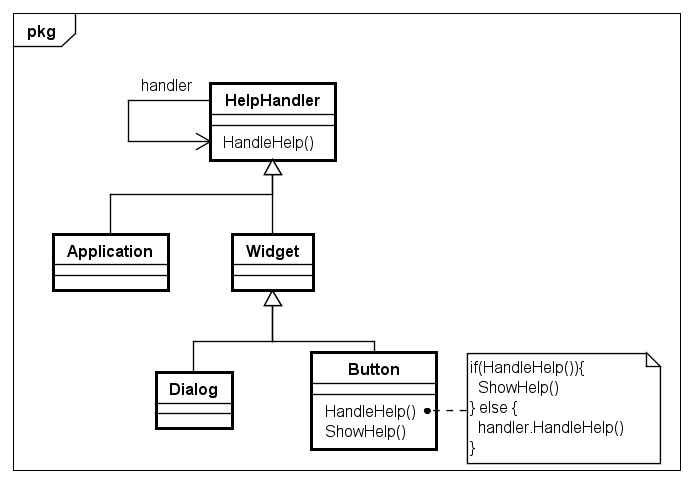
\includegraphics[scale=0.5]{5_padroes-contexto-funcional/5.3_comportamentais/5.3.01_chain-of-responsibility/chainofresponsibility_exemplo.png}
	\end{center}
\end{figure}

\begin{lstlisting}[caption={Chain of Responsibility Orientação a Objetos},label=oochresponsibility]

class HelpHandler(handler: HelpHandler = null, topic : Topic.Value = Topic.NO_HELP_TOPIC) {

  private var _handler : HelpHandler = handler
  private var _topic : Topic.Value = topic

  def HasHelp(): Boolean = {
    _topic != Topic.NO_HELP_TOPIC
  }

  def SetHandler(handler : HelpHandler, topic : Topic.Value) : Unit = {
    this._handler = handler
    this._topic = topic
  }

  def HandleHelp() : Unit = {
    if(_handler != null){
      _handler.HandleHelp()
    }
  }
}

class Widget(parent : Widget, topic : Topic.Value = Topic.NO_HELP_TOPIC)
  extends HelpHandler(parent, topic)
  
class Button(parent : Widget, topic: Topic.Value = Topic.NO_HELP_TOPIC)
  extends Widget(parent, topic) {

  override def HandleHelp(): Unit = {
    if(HasHelp()){
      //Oferece ajuda sobre o botão
    } else {
      parent.HandleHelp()
    }
  }
}

class Dialog(handler : HelpHandler, topic : Topic.Value = Topic.NO_HELP_TOPIC)
  extends Widget(null) {

  SetHandler(handler, topic)

  override def HandleHelp(): Unit = {
    if(HasHelp()) {
      // Oferece ajuda sobre dialog
    } else {
      handler.HandleHelp()
    }
  }
}

class Application(topic: Topic.Value)
  extends HelpHandler(null, topic) {

  override def HandleHelp(): Unit = {
    //Apresenta uma lista de tópicos de ajuda
  }
}

\end{lstlisting}

\subsection*{Contexto Funcional}

O Chain of Responsability encadeia funções que 
tratam solicitações, de forma que uma próxima 
função seja chamada quando a solicitação não 
pode ser tratada. É possível implementá-lo 
utilizando funções de alta ordem, onde um 
\textit{handler} é uma função, ao invés de 
uma classe, que armazena em uma \textit{closure} 
a função do próximo elemento da cadeia. 

O código \ref{fpchresponsibility} demonstra a 
criação dos \textit{handlers}. Na linha 2, a 
função HandleButton recebe como parâmetro um 
tópico e o próximo \textit{handler} da cadeia, 
assim como a classe Button do exemplo orientado 
a objetos. Ela retorna uma função que verifica 
se a solicitação pode ser tratada e, caso 
não seja, chama o \textit{handler} armazenado. 
A função HandleDialog, na linha 12, é 
implementada de forma análoga. Já a função 
HandleHelp, na linha 22, não recebe novos 
\textit{handlers}, oferecendo ajuda de forma 
genérica, da mesma forma que a classe 
Application do exemplo orientado a objetos.

\begin{lstlisting}[caption={Chain of Responsibility Funcional},label=fpchresponsibility]
    
def HandleButton(topic : Topic.Value, handler : () => Unit) : () => Unit = {
  () => {
    if(HasHelp(topic)){
      //Oferece ajuda sobre o botão
    } else {
      handler()
    }
  }
}

def HandleDialog(topic : Topic.Value, handler : () => Unit) : () => Unit = {
  () => {
    if(HasHelp(topic)){
      //Oferece ajuda sobre o dialog
    } else {
      handler()
    }
  }
}

def HandleHelp() : Unit = {
  //Apresenta uma lista de tópicos de ajuda
}
    
\end{lstlisting}

O código \ref{fpchainfunction} demonstra a criação 
da cadeia, onde as funções apresentadas anteriormente 
são executadas e encadeadas, criando a função 
ChainofResponsibility que será utilizada para 
tratar todas as solicitações.

\begin{lstlisting}[caption={Função Chain of Responsability},label=fpchainfunction]
    
val ChainofResponsibility: () => Unit = HandleButton(Topic.BUTTON,
  HandleDialog(Topic.DIALOG,
    HandleHelp))
      
\end{lstlisting}